% Osdag Design and Detailing Check List (DDCL)
% Beam to Column End Plate Moment Connection 
% Author: Ajmal Babu M S
\documentclass[11.5pt,a4paper,oneside]{report}
\usepackage{titlesec}
\setcounter{secnumdepth}{4}
\titleformat{\paragraph}
{\normalfont\normalsize\bfseries}{\theparagraph}{1em}{}
\titlespacing*{\paragraph}
{0pt}{3.25ex plus 1ex minus .2ex}{1.5ex plus .2ex}
\usepackage{graphicx}
\usepackage{url}
\usepackage{palatino}
\usepackage{tabularx}
\fontfamily{SansSerif}
\usepackage[T1]{fontenc}
%\usepackage[T1]{fontenc}
%\usepackage[latin1]{inputenc}
\usepackage{amsmath}
\usepackage{amsfonts}
\usepackage{amssymb}
%\usepackage{graphicx}
\usepackage{siunitx}
%\usepackage{tabularx}
\usepackage{algorithm2e}
\usepackage[top=1in, bottom=1in, left=0.8in, right=0.6in]{geometry}
\usepackage{fancyhdr}
%\usepackage{fancyheadings}
\usepackage{multirow}
\usepackage[bookmarks=false]{hyperref}   % For creating hyperlinks
\usepackage{comment}

\makeatletter
\makeatother
\hypersetup{
    colorlinks=true,
    linkcolor=blue,
    filecolor=magenta,      
    urlcolor=blue,
}
%======================================================
%					New Commands
%++++++++++++++++++++++++++++++++++++++++++++++++++++++
% To make the manual calculaion document, comment out following section
% and uncomment next section.
%------------------------------------------------------
%\newcommand{\okornot} { 
%	\vspace{15mm} \hrule \vspace{5mm}
%	\underline{Calculations} \\ \\ \noindent 
%	\TextField[name=multilinetextbox, multiline=true, width=1.0\linewidth,height=4in]{}} 
%------------------------------------------------------
\newcommand{\okornot}{ \vspace{15mm} \hrule
	\noindent \\ \\
	Is this check \qquad
	\CheckBox[checked=False, name= ok]{\textbf{Ok}} \qquad / 
	\CheckBox[checked=False, name= notok]{\textbf{Not Ok}}\\ \\
	Comments \\ \\
	\noindent
	\TextField[name=multilinetextbox, multiline=true, width=1.0\linewidth,height=2in]{}}
%++++++++++++++++++++++++++++++++++++++++++++++++++++++
% References for the check
\newcommand{\checkrefernces} {
	\vspace{15mm} \hrule \vspace{2mm}
	\textit{References:}}
%++++++++++++++++++++++++++++++++++++++++++++++++++++++
% Change 'Chapter' to 'Check'
\renewcommand{\chaptername}{Check}
%======================================================
%------------------------------------------------------
\begin{document}
	\title{Osdag\\ Open steel design and graphics}
	\author{Ajmal Babu M S}
	\date{07 August 2018}
\pagestyle{fancy}
\lhead{}
\chead{}
\rhead{\bfseries Moment Connection Module}
\lfoot{Osdag - Open steel design and graphics}
\cfoot{}
\rfoot{\thepage}
\renewcommand{\headrulewidth}{2pt}
\renewcommand{\footrulewidth}{1pt}
\newcommand{\univ}{Indian Institute of Technology, Bombay}
%------------------------------------------------------
\begin{titlepage}
	\begin{center}
		\begin{center}
			
\includegraphics {logoOsdag.png}
		\end{center}
			{\LARGE {Design and detailing checklist (DDCL)}}\\
			\vspace{1cm}
			{\LARGE {Beam to column end plate  moment connections}} \\
			\vspace{1cm}		
			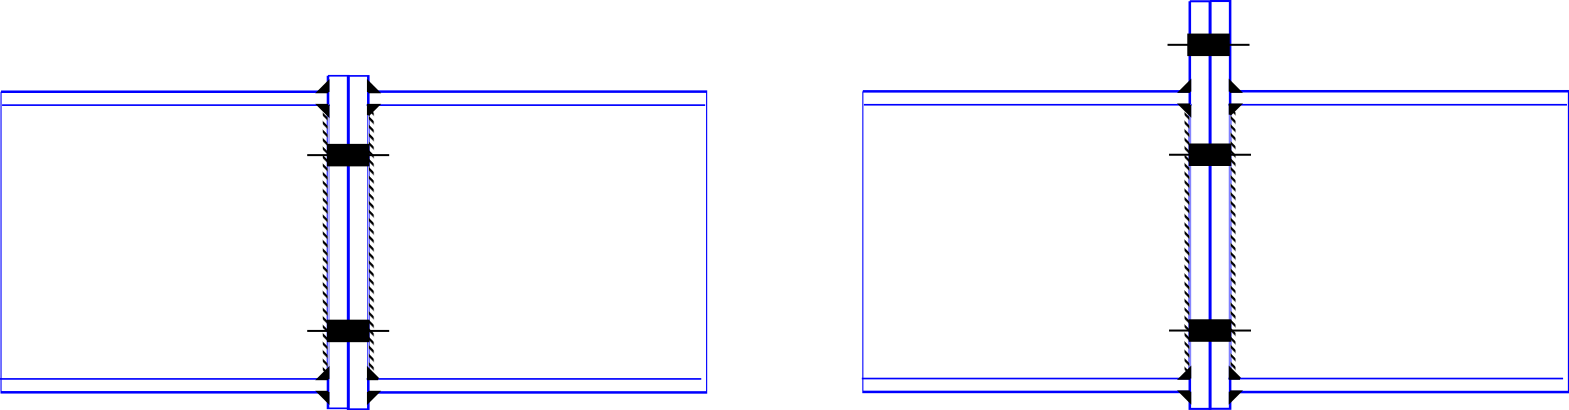
\includegraphics[width=7in]{FP_OWE.png} \\	
			\vspace{3cm}
			 {\small {Prepared by:}} \\
			 {\Large \textbf {Ajmal Babu M S}} \\	
			\vspace{0.5cm}	
			{\small {Under the guidance of} }\\
			{\Large \textbf {Prof. Siddhartha Ghosh}} \\	
			\vspace{1cm}
			\centering
			
\includegraphics[width=1.2in]{logo.png} \\	
 			\vspace{0.5cm}
			{\univ} \\ 
			\vspace{0.15cm}		
			{August 2018}
	\end{center}
\end{titlepage}
%------------------------------------------------------
\tableofcontents
\begin{Form}
%------------------------------------------------------
\pagenumbering{arabic}
\chapter*{Guideline for filling DDCL}
	\begin{itemize}
			\item    Guideline1
			\item    Guideline2
	\end{itemize}
%------------------------------------------------------
\chapter*{Reviewer Details}

%------------------------------------------------------
\chapter*{User Inputs}
%
\begin{itemize}
	\item Connecting members
		\subitem Connectivity*
		\subitem Beam Section*
		\subitem Column Section*
		\subitem $f_u$ (MPa)* 
		\subitem $f_y$ (MPa)* 
	\item Factored loads
		\subitem Moment (kNm)*
		\subitem Vert. Shear (kN)*
		\subitem Axial Force (kN)
	\item Bolt
		\subitem Diameter (mm)*
		\subitem Type *
		\subitem Grade *
	\item Plate
		\subitem Thickness (mm)*
		\subitem Height (mm)
		\subitem Width (mm)
	\item Weld size
		\subitem Flange weld (mm)*
		\subitem Web weld (mm)*
\end{itemize}
%=====================================================
\part*{Design and Detailing Checks}
%------------------------------------------------------
\chapter{Connecting Members}
%
The column and beam are allowed to connect by following connectivites.
\begin{itemize}
	\item Column flange to beam web
	\item Column web to beam web
\end{itemize}
%
The column and beam sections are provided as a dropdown list in Osdag input dock. Tapered sections from IS 808:1989 and parallel flange sections from the upcoming version of IS 808 are included. Old sections are highlighted in red colour in the dropdown with a warning that "user is using an old section which is not available in latest version of IS 808" in the message log.
%------------------------------------------------------
%\section{Connectivity}
%------------------------------------------------------
%
\section{Column Section}
%
All the columns sections are shown in dropdown.
%------------------------------------------------------
\section{Beam Section}
%
For column flange to beam web connectivity, 
\begin{equation}
	w_{bf} \le w_{cf}
\end{equation}
%
For column web to beam web connectivity,
\begin{equation}
	w_{bf} \le d_c - 2 (t_{cf} + r_{c1} + gap)
\end{equation}
Where, \\
\indent $w_{bf}$ = Width of beam flange \\
\indent $w_{cf}$ =  Width of column flange \\
\indent $d_c$ = Depth of column \\
\indent $t_{cf}$ = Thickness of column flange \\
\indent $r_{c1}$ = Root radius of column \\
\indent $gap$ = Clearance between beam and column flanges, 5mm


\okornot
%------------------------------------------------------
%					Material strength
%------------------------------------------------------
\chapter{Material Strength}
%
The column, beam and end plate are supposed to have the same strengths following the Indian Standards. The grades available in IS 800:2007 and IS 2062:2010 are included with a warning that "user is using a section of grade which is not available in the latest version of IS 2062". The values of material strength will be subjected to the following limits in \textbf{MPa};
\section{Yield Stress limits}
\qquad \qquad[Reference: Table-1, IS 800 : 2007; Table-2, IS 2062 : 2011]
	\begin{equation}
		250 \leq f_{y} \leq 650
	\end{equation}
\section{Ultimate Stress limits}
\qquad \qquad[Reference: Table-1, IS 800 : 2007; Table-2, IS 2062 : 2011]
	\begin{equation}
		410 \leq f_{u} \leq 780
	\end{equation}

	\okornot
%------------------------------------------------------
%					Factored Loads
%------------------------------------------------------
\chapter{Factored loads}
%
Factored values of the moment (in kNm) and vertical shear force  (in kN) acting on connection is mandatorily taken from the user. An optional field for axial force (in kN) is also given in the input dock if it is acting.\\
Assuming the beam is laterally supported and factored shear force does not exceed 0.6 times its design shear strength, 
The minimum moment capacity of connection,

\section{Minimum Factored Moment} 
\qquad \qquad[Reference: Cl. 10.7, b-1, IS 800 : 2007] \\ \\
	\begin{equation}\label{eq:cl_10.7b, IS 800}
		M_{min} = 0.5 M_d 
	\end{equation}
	Where, \\
		\indent $M_{min}$ = Minimum moment capacity of the connection \\
		\indent $M_d$ = Design bending strength of the beam, given by
	\begin{equation} \label{eq:cl_8.2.1.2a, IS 800}
		M_d = \beta_b Z_p f_y / \gamma_{m0} \le 1.5 Z_e f_y / \gamma_{m0} 
	\end{equation}
	Where, \\
		\indent $\beta_b$ = 1.0 for plastic and compact sections;\\
		\indent $\beta_b$ = $Z_e/Z_p$ for semi-compact sections;\\
		\indent $Z_p, Z_e$ = Plastic and elastic section modulii of the cross-section, respectively; \\
		\indent $f_y$ = Yield stress of the material; and;\\
		\indent $\gamma_{m0}$ = Partial safety factor \\
		\indent $M_{min}$ = Minimum moment capacity of the connection

\okornot
%------------------------------------------------------
%					Bolt
%------------------------------------------------------
\chapter{Bolt}
%
The diameter [from a dropdown list with 12, 16, 20, 24, 30 or 36 mm conforming to IS 1363 (part 1) 2002], type of bolt action (bearing or friction grip) and grade of bolts are taken from the user as inputs. The nominal tensile strength of bolt [IS 1367 (part 3): 2002] is considered as the ultimate tensile strength by default, and the user is allowed to overwrite it in 'Design Preference'. The bolt hole type is taken as 'Standard' by default and the user is allowed to change it to 'Over-sized' in 'Design Preferences,' and the bolt hole diameter is calculated accordingly, conforming to cl. 10.2.1 of IS 800:2007. The coefficient of friction (for friction grip bolts) is taken as 0.3 by default and the user is allowed to change it from a dropdown list with values given in table 20 of IS 800:2007. 
%======================================================
\section{Bolt Value}
%------------------------------------------------------
\subsection{Bearing type bolts}

\subsubsection{Design strength of bolt (\boldmath $V_{db}$)}
\qquad [Reference: Cl. 10.3.2, IS 800:2007] \\ \\ 

\noindent The design strength of bolt is taken as the smaller of the value as governed by shear, $V_{dsb}$ (\ref{shear_capacity}) and bearing $V_{dpb}$ (\ref{bearing_capacity}).

\begin{equation}
	V_{db} = min~ (V_{dsb}, V_{dpb})
\end{equation}

%------------------------------------------------------
\paragraph{Shear capacity (\boldmath $V_{dsb}$)}
\label{shear_capacity}
\qquad \qquad [Reference: Cl. 10.3.3, IS 800:2007] \\ \\
Currently, conservatively assuming all the shear planes passes through the threads of the bolt. Shear capacity of bearing bolts,
\begin{equation}
	V_{dsb} = \frac{f_u n_n A_{nb}}{\sqrt{3} \gamma_{mb}} \beta_{lj} \beta_{lg} 
\end{equation}
Where, \\
%\indent $V_{dsb}$ = design strength of bolt, as governed by shear strength;\\
\indent $f_u$ = ultimate tensile strength of a bolt;\\
\indent $n_n$ =  number of shear planes with threads intercepting the shear plane; \\
\indent $A_{nb}$ = net shear area of the bolt at threads, may be taken as the area corresponding to root diameter at the thread;\\
\indent $\gamma_{mb}$ = partial safety factor for bolt\\
\indent $\beta_{lj}, \beta_{lg}$ = factors, given by;

\begin{equation}
	\beta_{lj} = 1.075 - 0.005(l_j/d)
\end{equation}

\begin{equation}
	\beta_{lg} = 8/(3 + l_g/d)
\end{equation}

Where, \\
\indent $l_J$ = length of joint (measured in the direction of load transfer); \\
\indent $l_g$ = total thickness of the connected plates (grip length); \\
\indent $d$ = nominal diameter of the bolt. \\
%------------------------------------------------------
\paragraph{Bearing capacity (\boldmath $V_{dpb}$)}
\qquad \qquad [Reference: Cl. 10.3.4, IS 800:2007] \\ \\
\label{bearing_capacity}
\begin{equation}
	V_{dpb} = \frac{2.5~ k_b~ d~ t~ f_u}{\gamma_{mb}}
\end{equation}
Where, \\
\indent $k_b$ is smaller of $\frac{e}{3~d_0}, \frac{p}{3~d_0} - 0.25, \frac{f_{ub}}{f_u}, 1.0$; \\
\indent $e, p$ = end and pitch distances of the bolt along bearing direction; \\
\indent $d, d_0$ = diameter of bolt and bolt hole; \\
\indent $t$ = summation of the thicknesses of the connected plates experiencing bearing stress in the same direction; \\
\indent $\gamma_{mb}$ = partial safety factor.
%------------------------------------------------------
\subsubsection{Tension capacity (\boldmath $T_{db}$)}
\qquad \qquad [Reference: Cl. 10.3.5, IS 800:2007] \\ \\
\begin{equation}
T_{db} = \frac{0.90~ f_{ub}~ A_n}{\gamma_{mb}}~ < \frac{~f_{yb}~ A_{sb}}{\gamma_{m0}}
\end{equation}
Where, \\
\indent $f_{ub}$ = ultimate tensile stress of the bolt; \\
\indent $f_{yb}$ = yield tensile stress of the bolt; \\
\indent $A_n$ = net tensile stress area of the bolt; \\
\indent $A_{sb}$ = shank area of the bolt; \\
\indent $\gamma_{mb}, \gamma_{m0}$ = partial safety factors. \\
%------------------------------------------------------
\subsection{Friction grip type bolts}
%------------------------------------------------------
\subsubsection{Slip resistance (\boldmath $V_{dsf}$)}
\qquad \qquad [Reference: Cl. 10.4.3, IS 800:2007] \\ \\
\begin{equation}
	V_{nsf} = 0.7 \mu_f n_e  K_h A_{nb} f_{ub} / \gamma_{mf}
\end{equation}
Where, \\
\indent $\mu_f$ = coefficient of friction (slip factor); \\
\indent $n_e$ = number of effective interfaces offering frictional resistance to slip; \\
\indent $K_h$ = 1.0 for bolts in clearance holes and 0.85 for bolts in oversized holes; \\
\indent $F_o$ = proof load; \\
\indent $\gamma_{mf}$ = partial safety factor.
%------------------------------------------------------
\subsubsection{Tension capacity (\boldmath $T_{df}$)}
\qquad \qquad [Reference: Cl. 10.4.5, IS 800:2007] \\ \\
\begin{equation}
T_{df} = \frac{0.9~ f_{ub}~ A_n}{\gamma_{mf}} ~\leq~ f_{yb} A_{sb}  \frac{\gamma_{m1}}{\gamma_{m0} \gamma_{mf}}
\end{equation}
Where, \\
\indent $f_{ub}$ = ultimate tensile stress of the bolt; \\
\indent $f_{yb}$ = yield tensile stress of the bolt; \\
\indent $A_n$ = net tensile stress area of the bolt; \\
\indent $A_{sb}$ = shank area of the bolt; \\
\indent $\gamma_{m1}, \gamma_{mf}$ = partial safety factors. \\

%======================================================
%------------------------------------------------------
%======================================================
\section{Minimum Number of bolts}
%------------------------------------------------------
Minimum number of bolts required is calculated based on the tension acting on bolts. A 20~\% reduction on bolt tensile capacity is assumed to account the prying force. Total number of bolts in the configuration is determined based on the layouts given in Sec. \ref{layout} \\
Minimum number of bolts required at the tension side, $n_f$

\begin{equation}
	n_f = \frac{T_f}{0.8 * T_b}
\end{equation}

Where, \\
\indent $T_b$ = tension capacity of bolts \\
\indent $T_f$ = tension in flange, claculated as; \\

\begin{equation}
	T_{f} = \frac{M_u}{D - t_f} ~ + ~ \frac{H}{2}
\end{equation}

Where, \\
\indent $M_u$ = factored bending moment acting on the connection. \\
\indent $D$ = depth of the beam; \\
\indent $t_f$ = thickness of the beam flange; \\
\indent $H$ = axial force acting on the connection. \\

\section{Layout of Bolts}
\label{layout}
\begin{figure}[h]
	\centering
	\includegraphics[height=0.9\textheight]{test.png}
\end{figure}


**add images
%------------------------------------------------------
%					Detailing
%------------------------------------------------------		
\chapter{Detailing}
	{\centering
	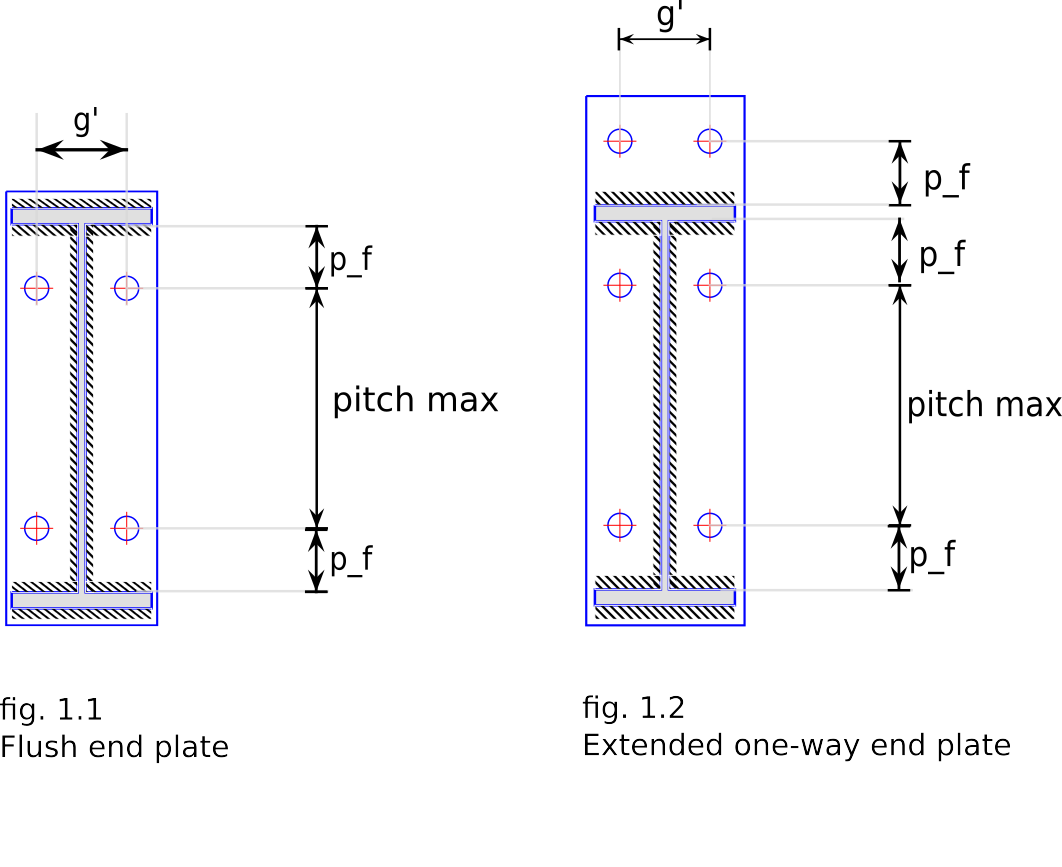
\includegraphics[width=5in]{svg_drawingFPEOW.png} \\}

\section{Pitch and guage distances}
	Pitch (p) is the distance between centres of two adjacent fasteners in a line lying in the direction of stress.
	Guage (g) is the distance between centres of two adjacent fasteners transverse to the direction of stress.

\subsection{Minimum pitch and guage distances}
	\indent [Reference: Cl. 10.2.2, IS 800 : 2007]\\
		\begin{equation}
			 \textbf{\,pitch/gauge} \ge 2.5 * bolt\, diameter
		\end{equation}
				
\subsection{Maximum pitch and guage distances}
\indent [Reference: Cl. 10.2.3, IS 800 : 2007]\\				
		\begin{equation}
			\textbf{\,pitch/gauge \,} \leq min(32 * t,\, 300\, mm)
		\end{equation}
		where, \\
			\qquad t = thickness of thicker plate being connected 

\section{End and egde distance}
				
		\large {End (e)/ Edge (e') distance (\textbf{already reviewed}) [Reference: Clause 10.2.4, IS 800 : 2007]} \\
				%\vspace{5mm}
				\begin{equation}
				\boxed{ 1.7 * bolt\,hole\, diameter\, \leq \textbf{\,end/edge \,} \leq 12*t*\varepsilon }
				\end{equation}
				
				\hspace{10mm}
				where,
				
				\hspace{30mm}
				t = thickness of thicker plate being connected
				
				\hspace{30mm}
				$\varepsilon = (250 / f_{y}) ^ {(1/2)}$ 
				
				\hspace{30mm}
				$f_{y}$ = yield strength of beam/plate material 				 
			
			\vspace{2mm}
				
\section{Cross-centre gauge distance (g')} 
(\textbf{refer fig. 1.1 and 1.2}) \\

		\subsubsection{Flush end plate}
		[Reference: AISC Design Guide - 16, table 3-6, page 22]
		\begin{equation}
		\boxed{ 57 mm \leq \textbf{g'} \leq 95 mm }
		\end{equation}
		
		\subsubsection{Extended one way}
		[Reference: AISC Design Guide - 16, table 4-7, page 39]
		\begin{equation}
			\boxed{ 69 mm \leq \textbf{g'} \leq 177 mm }
		\end{equation}

\section{Distance between centre of bolt and edge of the beam flange ($p_{f}$)}

 (\textbf{refer fig. 1.1 and 1.2})\\
				
					\subsubsection{Flush end plate}
						[Reference: AISC Design Guide - 16, table 3-6, page 22]
						\begin{equation}
							\boxed{ 33 mm \leq p_{f} \leq 47 mm }
						\end{equation}
						
						\subsubsection{Extended one way}
						[Reference: AISC Design Guide - 16, table 4-7, page 39]
						\begin{equation}
							\boxed{ 25 mm \leq p_{f} \leq 38 mm }
						\end{equation}

	    

%------------------------------------------------------
%					Plate Dimensions
%------------------------------------------------------	
\chapter{Plate Dimensions} 
\section{Plate height $(h_{p})$}
				
 \large {$h_{p}$ for flush end plate}
					\begin{equation}
					\boxed{h_{p} = beam\, depth + (2 * size\, of\, weld\, at\, flange) + (2 * some\, assumed\, cover)}
					\end{equation}
		
\large {$h_{p}$ for extended one-way end plate}
					\begin{equation}
					\boxed{h_{p} = beam\, depth + end\, distance + p_{f} + size\, of\, weld\, at\, \,flange + some\, assumed\, cover}
					\end{equation}
					
			
\section{\large Plate width $(w_{p})$}
			
				\begin{equation}
					\boxed{w_{p} = width \,of \,beam \,flange}
				\end{equation}

\section{Thickness of the plate $(t_{p})$}

Plate thickness for flush end plate
	
	

%------------------------------------------------------
%					Weld
%------------------------------------------------------	
\chapter{Weld} 
\section{Weld size}
\subsection{Flange weld}
\subsection{Web weld}
\section{Weld length}
%------------------------------------------------------
%------------------------------------------------------
\end{Form}
\end{document}
